\chapter{Literature review}\label{chapt:lit}
\section{Convolutional Neural Networks(CNN)}
[\textit{A CNN is a type of Artificial neural network(ANN) where convolutional blocks are used instead of basic 1-D multilayer perceptrons}]

For understanding CNN, we need to see what an artificial neural network(ANN) is. ANN is a system of interconnected neurons used to model complex functions for classification and regression. Any model is made up of at least three layers: An input layer, one or more hidden layers, and an output layer. The most basic ANN model consists of multilayer perceptrons. \ref{subsection:types_of_layers} shows different types of layers that can be used for a convolutional neural network. Several nonlinear activation functions such as rectified linear unit (ReLU)or sigmoid, or even custom functions can be applied at any point on the layers to produce activation maps. These activation maps finally help us in classification or segmentation.

\subsection{Types of layers}
\label{subsection:types_of_layers}
The general structure of any convolutional neural network can be categorized as follows:
\begin{enumerate}[(a)]
    \item \textbf{Input layer}:
        The input layer is the input of any neural network. The input of computer vision problems is usually an image that is basically a matrix of numbers stacked multiple times(channels). An RGB image has 3 channels[Figure~\ref{fig:RGB_image}].
        \begin{figure}[h!]
            \centering
            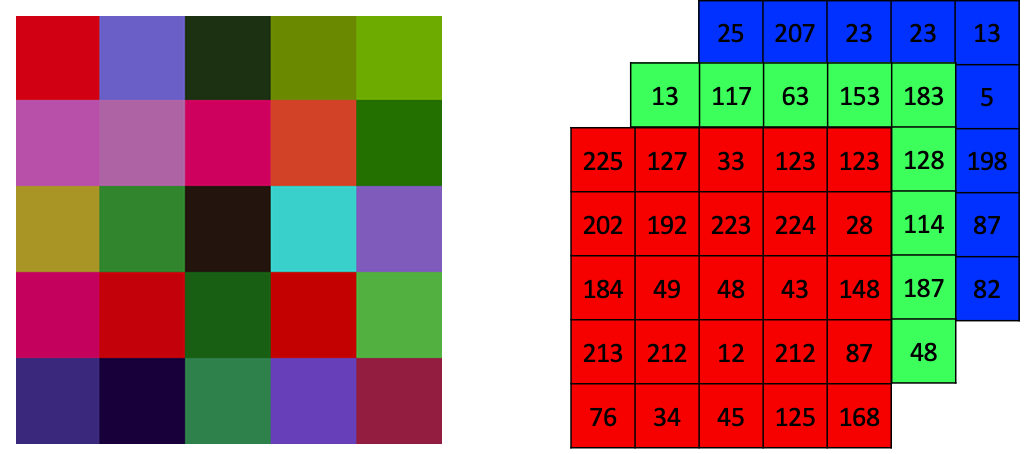
\includegraphics[width=0.8\textwidth]{rgb_image_as_array}
            \caption[RGB image shown as matrix]{RGB image shown as matrix. Resolution of this image is $5\times5$.}
            \label{fig:RGB_image}
        \end{figure}
        
    \item \textbf{Convolution layer}:
        As the name suggests, this is the most important layer of convolutional neural networks. A convolutional layer contains a set of filters(or kernel or node) whose parameters need to be learned. The height and width of the filter are predefined when defining the layer and are smaller than those of the input volume. For most images, the dimension of the filter is taken $3\times3$ or $5\times5$, but if the given image is large, filters up to size $11\times11$ can also be used. One catch is: a filter is not two dimensional. It takes in the dimension of the input it is provided with.

        Applying a filter to an image means taking the inner product of the image and the filter within the overlapping area, which keeps on moving. Suppose the dimension of an image is $W\times W$ and dimension of the filter is $k\times k$, the dimension of the output image will be $(W-k+1)\times (W-k+1)$. Once a filter has been applied, it passes through an activation function, and the resulting image is called the output of that filter.
    
        The formula for convolutional neural network is: \begin{equation} a_{i,j} = f(\Sigma_{m=0}^2\Sigma_{n=0}^2 W_{m,n}X_{m+i,n+j}) \end{equation} where $\text{X}_{i, j}$ represents the pixel value of line $i$ in column $j$ of the image and $W_{m, n}$ represents the weight of column $n$in row $m$. Similarly, $a_{i,j}$ represents the value of column $j$ of the $i$ row of the feature map; the activation function is represented by $f$. [Example: Figure~\ref{fig:convolution_filter_process}].
        \begin{figure}[h!]
            \begin{subfigure}[b]{0.35\textwidth}
            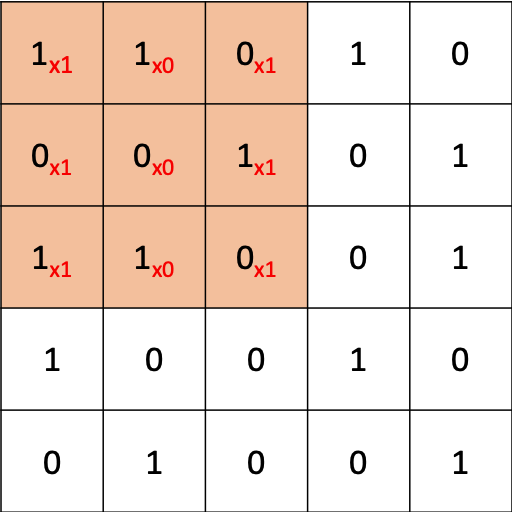
\includegraphics[width=\textwidth]{cnn_filter_input}
            \caption{}
            \end{subfigure}~
            \begin{subfigure}[b]{0.2\textwidth}
            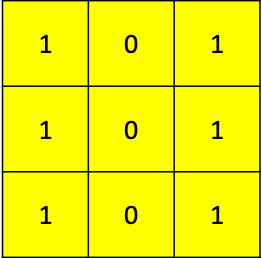
\includegraphics[width=\textwidth]{cnn_filter}
            \caption{}
            \end{subfigure}~
            \begin{subfigure}[b]{0.2\textwidth}
            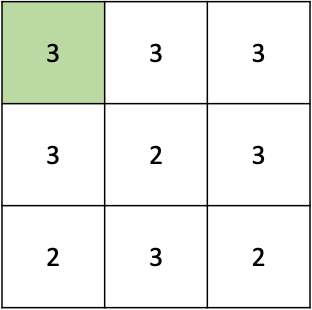
\includegraphics[width=\textwidth]{cnn_filter_convolution}
            \caption{}
            \end{subfigure}~
            \begin{subfigure}[b]{0.2\textwidth}
            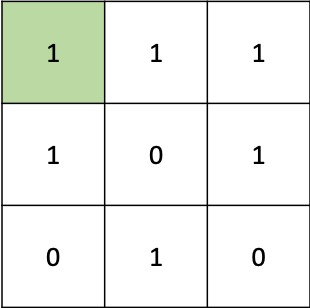
\includegraphics[width=\textwidth]{cnn_filter_output}
            \caption{}
            \end{subfigure}
            \caption[The process of convolution]{The process of convolution: (a) Input vector. (b) Filter being convoluted on (a). (c) Result of (b) convoluting over (a). (d) Final result after applying activation function $a_{i,j}>2$.}
            \label{fig:convolution_filter_process}
        \end{figure}

        Each filter in the convolution layer uses the output of the previous layer to connect and calculate. The number of filters is predefined and usually kept in powers of 2. Suppose a layer has 64 filters of dimension $3\times3$, the input image has dimensions of $1000\times1000$, the resulting output will be of dimension $998\times998\times64$. If this is passed into another layer consisting of 128 filters and the same dimension, the new output will be $996\times996\times128$.

    \item \textbf{Pooling layer}:
        The amount of data after the multilayer convolution layer is huge. To reduce the time taken for calculations, we need to reduce the size of the matrix. This means we need to reduce the number of parameters of the fully-connected layer. This is done by using a pooling layer. The pooling layer finds the eigenvalues of the image, which are then used as the basis of classification. The pooling layer also prevents data from overfitting.

        The pooled layer function similar to data resampling. The filter propagates in the same way as the filters in the convolution layer. The difference between the two is that instead of taking the inner product with the filter, we take the maximum or average value of the window. The most used pooling methods are max pooling, mean pooling, and random pooling layers. In a max-pooling layer, the maximum value of a pre-specified window replaces the given dataset. If the dataset is replaced by averaging the contents in the window, it is called an average pooling layer. A number is selected randomly according to the probability matrix in random pooling.

    \item \textbf{Fully connected layer}:
        Unlike the filters in the convolution layer where only some pixels are taken into account, each fully connected layer uses the previous layer's global information. This means each node’s calculation is connected with the weights of all nodes in the previous layer. This is the reason this layer is usually used at the end of the model. 

        Because it takes in the global context, this means the complete information received from convolution and pooling operations is taken into consideration for output from this layer. Given the outputs, an activation function is applied for classification purposes.
\end{enumerate}

% There are some special types of convolutional layers which perform specific tasks:
\subsection{Dilated convolution}
[\textit{Convolution with dilated filter; Also called atrous convolution}]

    Dilated convolutional layers are used in image segmentation, where its class labels each pixel. As the name suggests, Dilated convolution is basically dilating the filter before doing the usual convolution. Dilating the filter means expanding, taking in distant elements instead of the adjacent elements in the input matrix to calculate weights. These filters are also called upsampled filters. The empty positions in between are filled with zeros, thus making this kind of sparse matrix. The distance in a Dilated convolution filter is determined by the dilation coefficient D(Also called dilation rate). If the dilation rate is 1, it means it is the standard convolutional kernel. If the dilation rate is 2, then there is a skip of one pixel per input. In general, if there is a dilation rate of n, skip of n-1 pixels per input.
    
    Figure~\ref{fig:dilated_layer} shows how the kernel elements are matched to input elements in a D-dilated 3x3 convolution. Also notice how the dilated convolution layer has increased the spatial context(a.k.a feature maps or receptive field or the field of view) without decreasing the resolution of output.
    \begin{figure}
        \centering
        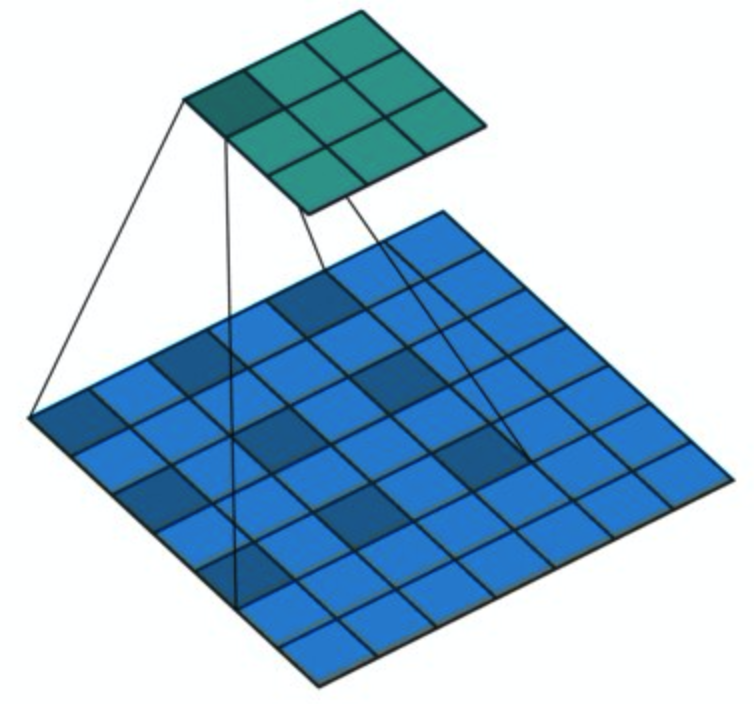
\includegraphics[width=0.5\textwidth]{cnn_dilated_layer}
        \caption[Dilated convolution layer]{Notice how dilated convolution layer increases the capture of spatial context. Dilation rate is 2 in this figure.}
        \label{fig:dilated_layer}
    \end{figure}


\subsection{Strided convolution}
    In a regular convolution, we usually shift the windows by 1 pixel. However, for some large images, it is necessary to shrink feature maps to make computations feasible. In stride convolution, we change the length of stride in each step. This means we skip some input values while performing convolution operations and thus decreasing the output dimension. In general, this operation does a trad off between resource consumption and information retrieval.


\section[Residual Blocks]{Residual Blocks - Going deeper into Convolutional Neural Networks}

In a neural network, weights receive an update proportional to the gradient of current weight in each iteration. \begin{equation} ChangeInWeight_{i} \propto \frac{\partial(ErrorFunction)}{\partial(weight_{i})} \end{equation} When the gradient of the training model becomes vanishingly small, the change in weight becomes negligible, and thus model training essentially stops. This problem is called the problem of vanishing gradient.

Conventionally, as the CNNs become deeper, the problems related to vanishing gradients became severe. To solve this problem, {Kaiming He, Xiangyu Zhang, Shaoqing Ren, Jian Sun}\cite{ResNet} developed the concept of residual networks(Also called ResNet or skip connections). Residual neural networks tackle vanishing gradients by skipping connections or making shortcuts to jump over some layers (Figure~\ref{fig:residual_network}). Typical ResNet models are implemented with double- or triple- layer skips that contain nonlinearities (ReLU) and batch normalization in between.

\begin{figure}[h!]
    \centering
    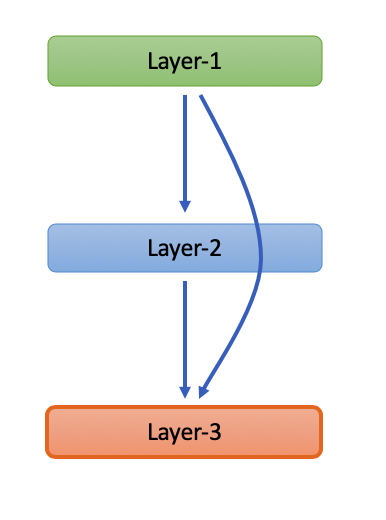
\includegraphics[width=0.2\textwidth]{lit_resnet}
    \caption[A residual network]{Canonical form of a residual neural network. Layer-2 is skipped over activation from Layer-1.}
    \label{fig:residual_network}
\end{figure}

While training, an additional matrix can be used to train the skip connections as well. These are usually identity matrices and not so hard on memory; hence they can be used to quickly train much deeper networks than what was achieved with the conventional neural networks. ResNet also increases performance while training the model. This is due to the face that some layers are essentially skipped, and the gradients that were earlier vanishing now converge faster.

Many improvements to the original ResNet architecture have been made since its inception. Pre-trained models like ResNet (34, 50, 101) are already available in popular libraries like Tensorflow and PyTorch. ResNet is considered one of the most significant innovations in the area of neural networks

\section{Encoder-Decoder}
The encoder-decoder architecture is the standard neural machine translation method that rivals and, in some cases, outperforms classical statistical machine translation methods.

Though this architecture is very new, having only been pioneered in 2014. The Encoder-Decoder architecture has become a modern approach for sequence-to-sequence (seq2seq) predictions. Road detection needs a sequence-to-sequence learning framework to keep track of spatial characteristics. It has three components: an encoder network, a decoder network, and an intermediate network.

% In a CNN, an encoder-decoder network typically looks like this (a CNN encoder and a CNN decoder):


% Image credits

% This is a network to perform semantic segmentation of an image. The left half of the network maps raw image pixels to a rich representation of a collection of feature vectors. The right half of the network takes these features, produces an output and maps the output back into the “raw” format (in this case, image pixels).


% An encoder is a network (FC, CNN, RNN, etc) that takes the input, and output a feature map/vector/tensor. These feature vector hold the information, the features, that represents the input. The decoder is again a network (usually the same network structure as encoder but in opposite orientation) that takes the feature vector from the encoder, and gives the best closest match to the actual input or intended output.

The encoders are trained with the decoders. There are no labels (hence unsupervised). The loss function is based on computing the delta between the actual and reconstructed input. The optimizer will try to train both encoder and decoder in such a way that the features that matter the most should have lower reconstruction loss. This also means that, given an encoded sequence, we do not try to reconstruct the actual input, but rather try to map inputs to specific outputs. For example, given a map, it maps roads to true and assigns everything else to false. This is how a Lossy compression algorithm helps us in the segmentation of an image.


% , essentially. Suppose you have a vector v that is represented by 11 values and you use an encoder to reduce that vector to being represented by 10 values through matrix/vector multiplication. Eigen Decomposition, Moore-Penrose Pseudoinverses. That sort of crap. The decoder transforms it back to 11 values, but an approximation of the original 11 values. I believe a simple form of the process is known as PCL. Data loss can be absolutely minimized for a known data set once the decoded approximation is calculated, and the encoder and decoder can be tuned appropriately.

% It consists of 3 parts: encoder, intermediate vector and decoder.




% Encoder-It accepts a single element of the input sequence at each time step, process it, collects information for that element and propagates it forward.

% Intermediate vector- This is the final internal state produced from the encoder part of the model. It contains information about the entire input sequence to help the decoder make accurate predictions.

% Decoder- given the entire sentence, it predicts an output at each time step.


% Encoder: Maps (sensory) 
% Decoder: 
% In a perfect Encoder plus Decoder network (also referred to as autoencoder) the input into the encoder is matching the output of the decoder, such that the network is able to reconstruct its own input.


% “Generally, the encoder encodes the input sequence to an internal representation called 'context vector' which is used by the decoder to generate the output sequence. The lengths of input and output sequences can be different, as there is no explicit one on one relation between the input and output sequences.”

% \section{Super Resolution}


% \section{Road Detection}
% It can be both binary and fuzzy

% \section{Training process of convolutional neural network}

% In this paper, the road extraction of remote sensing image is studied. Firstly, the convolutional neural network is used to classify the high-resolution remote sensing image, distinguish the road from the non-road, and extract the road information initially. Secondly, the convolutional neural network is optimized and improved from the training algorithm. In this section, the training process of convolutional neural network is improved to realize road classification in remote sensing images.

% Gradient descent algorithm is simple, easy to converge, but easy to fall into the local optimal solution, and the gradient descent near the saddle point is slow, affecting the training of network model. The saddle point can be avoided in the training process of Newton algorithm, but the method needs to compute Heisen matrix to ensure its non-negative positive definite and a large amount of storage space and to ensure the existence of second-order derivatives of the objective function; otherwise, it is difficult to ensure the convergence of the algorithm [26,27,28]. In order to avoid the difficulties caused by the direct use of the Newton algorithm, the improved BFGS quasi-Newton algorithm [29] is used to train convolutional neural networks.

% In the Newton algorithm training process, the CNN model parameters are updated to:
% 𝑊𝑖+1=𝑊𝑖−∇𝑗𝑤∇2𝑗𝑤
% (9)

% The initial quasi-Newton algorithm equation is:
% 𝐵𝑘+1𝑆𝑘=𝑦𝑘
% (10)

% where Sk = Wk + 1 − Wk, yk =  ∇ jw + 1 −  ∇ jw. In order to achieve better target optimization effect, the improved BFGS is used in this paper.
% 𝐻𝑘+1=𝐻𝑘+𝑦𝑘𝑦𝑡𝑘𝑦𝑡𝑘𝑠𝑘−𝐻𝑘𝑠𝑘𝑠𝑡𝑘𝐻𝑘𝑠𝑡𝑘𝐻𝑘𝑠𝑘
% (11)

% However, the Heisen matrix obtained by the recursion formula may be a singular matrix, and the inverse matrix calculation has a certain degree of complexity, so the recursion formula in this paper is expressed as follows:
% 𝐵−1𝑘+1=(𝐵0−𝑠𝑘𝑦𝑇𝑘𝑠𝑇𝑘𝑦𝑘)𝐵−1𝑘(𝐵0−𝑦𝑘𝑠𝑇𝑘𝑠𝑇𝑘𝑦𝑘)+𝑠𝑘𝑠𝑇𝑘𝑠𝑇𝑘𝑦𝑘
% (12)

% Based on the above theory and formula, the training process of the improved BFGS algorithm is as follows:

%     1.

%     Select iteration times epochs, epoch = 0, initialization parameter w and offset b.
%     2.

%     If epoch < epochs, iteration stops.
%     3.

%     Calculate the value of bkdk +  ∇ jw = 0 and get a new optimization direction 𝑑𝑘=−𝐵−1𝑘𝑔𝑘

%     .
%     4.

%     Search along the dk direction to satisfy wk + 1 = wk + akdk, it is the minimum point in this direction, ak > 0.
%     5.

%     Let the epoch iteration add 1 and go to (2).
